\documentclass{llncs}
\usepackage[T1]{fontenc}
\usepackage[utf8]{inputenc}
\usepackage[spanish]{babel}
\usepackage{graphicx}
\usepackage{graphics}
\DeclareGraphicsExtensions{.eps,.ps,.pdf}
\usepackage{url}
\usepackage{lscape}
\usepackage{eurosym}
 
\def\CC{{C\hspace{-.05em}\raisebox{.4ex}{\tiny\bf ++}}~}
\addtolength{\textfloatsep}{-0.5cm}
\addtolength{\intextsep}{-0.5cm}

%%%%%%%%%%%%%%%%%%%%%%%%%%%%%%%%%%%%%%%%%%%%%%%%%%%%%%%%%%%%%%%%%%%%%%%%%
\title{Studying individualised transit indicators in the metropolitan area of Granada using a new low-cost information system}  
%Obtención de indicadores de exposición mediante un nuevo sistema de información de bajo coste
%Estudio de los indicadores de exposición en el área metropolitana de Granada mediante un nuevo sistema de información de bajo coste

\author {
P.A. Castillo, P. García-Fernández, P. García-Sánchez, \\ M.G. Arenas, A.M. Mora, G. Romero, J.J. Merelo
}
\institute{
Department of Architecture and Computer Technology. CITIC \\
University of Granada (Spain) \\
~\\
e-mail: {\tt pedro@atc.ugr.es}
}


\date{}
\begin{document}
\renewcommand{\tablename}{Table }
\renewcommand{\figurename}{Figure }
\maketitle

\begin{abstract}

 % Dados los beneficios de un sistema de información sobre el estado del tráfico y del uso de la red viaria por parte de los vehículos, se plantea el desarrollo de un sistema de información de bajo coste y autónomo para monitorizar el tráfico y conocer el estado de las carreteras en tiempo real.
Given the benefits of an information system about the traffic intensity and about the usage of vehicles, in this paper, a new low-cost information system to monitor the traffic in real-time is proposed.

 % Los sistemas de información utilizados actualmente para la recopilación de datos y generación de información sobre el estado de las carreteras presentan dos inconvenientes: la primera es que no tienen capacidad para identificar e individualizar los vehículos que detectan. La segunda es su elevado coste, lo cual los hace caros para cubrir la red de carreteras secundarias, por lo que se suelen ubicar en vías principales y en salidas de grandes núcleos de población.
Current information systems used for data collection and to generate information on the state of the roads have two drawbacks: the first is that they have no ability to identify and target the vehicles detected. 
The second is their high cost, which makes them expensive to cover the secondary road network, so they are usually located just on main routes.

 % En este trabajo proponemos un sistema basado en el escaneo de los identificadores de dispositivos bluetooth que hay en el entorno. Se trata de un identificador único que permite saber el fabricante e incluso distinguir de qué tipo de dispositivo se trata (PC, teléfono móvil, equipo manos libres, etc).
In this paper we propose a system based on scanning bluetooth devices that are near the detection node. 
This is an unique identifier that allows to know the manufacturer and even distinguish what type of device it is (PC, mobile phone, handsfree, etc).

 % Pretendemos recoger gran cantidad de datos del paso de dispositivos bluetooth para buscar apariciones de un dispositivo en diferentes nodos (movimientos o desplazamientos), determinar la frecuencia de aparición, calcular velocidades de movimiento entre nodos o calcular el número de dispositivos que pasan por cierto sitio cada día (ya sea festivo o laborable).
We intend to collect large amounts of data from passes of bluetooth devices by different nodes (movements or displacements). Thus we could determine the frequency of appearance, calculate speeds between nodes, or calculate the number of devices that pass certain site each day (on both working or non-working days).

 % Obtendremos estadísticas y de este modo estudiaremos diversos indicadores relativos al uso de vehículos por parte de la población del área monitorizada.
Statistics will be obtained and thus several indicators relating to the use of vehicles by the population of the monitored area will be studied.


{\bf Palabras clave}: DGT, SINECA, traffic, exposure indicators, new technologies, bluetooth, monitoring

\end{abstract}


%\newpage


%%%%%%%%%%%%%%%%%%%%%%%%%%%%%%%%%%%%%%%%%%%%%%%%%%%%%%%%%%%%%%%%%%%%%%%%%
\section{Introduction}

 % Contar con un sistema de información sobre el estado del tráfico y del uso de la red viaria por parte de los vehículos se antoja clave en el contexto actual. Con una población cada vez más informada y con dispositivos de comunicación ubicuos que poseen y usan habitualmente prácticamente el $90\%$ de la población, obtener información sobre cómo se encuentra el tráfico en cualquier momento en cualquiera de los casi 20.000 kilómetros con los que cuenta la red viaria nacional, significaría poder gestionar de manera óptima una red de comunicaciones vital para un porcentaje elevado de usuarios. 
Having a system of information on traffic conditions and the use of roads by vehicles seems key in the current context. 
With a population increasingly informed, provided with communication devices ubiquitous commonly used about $ 90 \% $ of the population, obtaining information about the traffic in any of the nearly 20,000 kilometers of roads, would mean to optimally manage a communications network vital for a high percentage of users.

 % La aplicación de esta propuesta en el transporte supondrá disponer de un sistema de información sobre el estado del tráfico del uso de la red viaria por parte de los vehículos. 
The application of this proposal in the transportation system will involve having an information system on the traffic status.

 % Nuestro objetivo final es disponer de información acerca de los flujos de tráfico que se producen en cierta zona, lo que permitirá poder gestionar de manera óptima las decisiones de desplazamiento por parte de los ciudadanos. 
Our ultimate goal is to have information about traffic flows that occur in a certain area, allowing to optimally manage motion decisions by citizens.

 % Por tanto, encontramos que se tienen varias necesidades desde el punto de vista de la gestión del transporte:
Therefore, various needs from the viewpoint of the transport management have been found:

%\begin{itemize}
%  \item Se necesitará un dispositivo autónomo y versátil de recogida de datos y monitorización.
%  \item Además es necesario recopilar los datos del tráfico en tiempo real. 
%  \item Una vez se tienen los datos, hay que procesarlos de manera correcta para poder ofrecer la información específica necesaria.
%  \item Y por último, se necesita un sistema que teniendo en cuenta la evolución de los actuales sistemas de información, permita poder compartir esos datos con aquellos que toman decisiones sobre movilidad, no sólo desde el punto de vista institucional sino también desde el punto de vista personal.
%\end{itemize}

\begin{itemize}
  \item A versatile and autonomous data collection and monitoring device is needed.
  \item It is also necessary to collect traffic data in real time.
  \item Once the data has been collected, it has to be processed properly.
  \item And finally, a system that allows sharing data and information with those who make decisions about mobility is needed, both from the institutional and personal points of view.
\end{itemize}


 % En este trabajo presentamos un sistema basado en la detección de dispositivos bluetooth (BT). Concretamente se captarán las ondas que emiten los diferentes componentes tecnológicos que ya incorporan los vehículos (manos libres, gps), los accesorios que incorpora el usuario a un vehículo, así como los propios teléfonos móviles que llevan sus ocupantes.
In this work, a system based on bluetooth (BT) device discovery is proposed. 
Specifically, it will catch waves emitted by different technological components incorporated on vehicles (handsfree, gps), accessories that the users incorporate to their vehicles, as well as their mobile phones.
 % El principal dato que se recoge es la dirección MAC de la tarjeta BT de los dispositivos que pasan. 
 % Se trata de un identificador único para cada dispositivo, lo que nos permitirá individualizar los vehículos que pasan.
 % Desde el punto de vista de la privacidad de datos, hay que destacar que los datos recopilados no se asociarán a ningún usuario ya que no existe ningún tipo de información que haga posible la identificación de los datos que recopilamos con una persona en concreto. Para ello hacemos utilización de tecnologías de encriptacion unidireccionales con caracteres no estándar que imposibilitan identificar la MAC del dispositivo inalámbrico. De esta forma, la intrusividad al hacer la recopilación de datos es mínima.
The main data that is collected is the MAC address of the device BT card.
This is an unique identifier for each device, allowing us to identify passing vehicles.
From the point of view of data privacy, it is noteworthy that the data collected will not be associated to any user because there is no information that enables the identification of the information we collect with a specific person. 
Encryption technology unidirectional with nonstandard characters that preclude identifying the MAC of the wireless device is used. Thus, intrusiveness is minimal.
 % Recogeremos gran cantidad de datos del paso de dispositivos BT para obtener diferentes estadísticas y  estudiar diversos indicadores relativos al uso de vehículos por parte de la población del área monitorizada.
A large amount of data related to passing BT devices will be collected, to calculate statistics and to study several indicators about the use of vehicles by the monitored area population.

%El resto del trabajo está organizado como sigue:
%En la Sección \ref{soa} se recopilan las tecnologías utilizadas en la actualidad para monitorizar el tráfico que pasa por cierta zona.
%La Sección \ref{obj} detalla los objetivos planteados en este trabajo.
%En la Sección \ref{hw} se presenta el dispositivo de recopilación de datos Intelify, con el que ya se ha comenzado a trabajar.
%En la Sección \ref{analisis} se muestran los diferentes análisis que se han llevado a cabo a partir de los datos obtenidos a lo largo del proyecto.
%Por último, se presentan una serie de conclusiones y trabajos futuros (Sección \ref{conclus}).

The rest of the paper is organized as follows:
In Section \ref{soa} current technologies to monitor the traffic that passes through a certain area is summarized.
Section \ref{obj} details the goals of this paper.
In Section \ref{hw}, the Intelify device is presented.
In Section \ref{analisis} several analysis and statistics are reported from the data obtained.
Finally, we present some conclusions and future work (Section 5).


%%%%%%%%%%%%%%%%%%%%%%%%%%%%%%%%%%%%%%%%%%%%%%%%%%%%%%%%%%%%%%%
\section{Current technologies}
\label{soa}

Traffic detection technologies can generally be classified into two groups: intrusive and nonintrusive.

Intrusive detection technologies are installed on/within the roadway, which require lane closures. Using this type of technology is inherently more hazardous and is generally more time consuming, especially for temporary traffic data collection. This technology has a number of drawbacks:
\begin{itemize}
  \item Installation requires pavement cut.
  \item Improper installation decreases pavement life.
  \item Installation and maintenance require lane closure.
  \item Detection accuracy may decrease when design requires detection of a large variety of vehicle classes.
  \item Poor pavement condition can dramatically shorten the life span of intrusive sensors.
\end{itemize}

Non-intrusive technologies are traffic detection sensors that cause minimal disruption to normal traffic operations during installation, operation and maintenance compared to conventional detection methods. They can also be deployed more safely than conventional detection methods and are deployed adjacent to the roadway and require minimal interaction with traffic flow. These are mainly of two types: active (microwave radar, ultrasonic and laser radar), o passive (infrared, acoustic and video image processing). 

Figure \ref{tipossensores} shows a classification of information systems according to the intrusiveness of the technology.

\begin{figure}[htpb] 
\begin{center} 
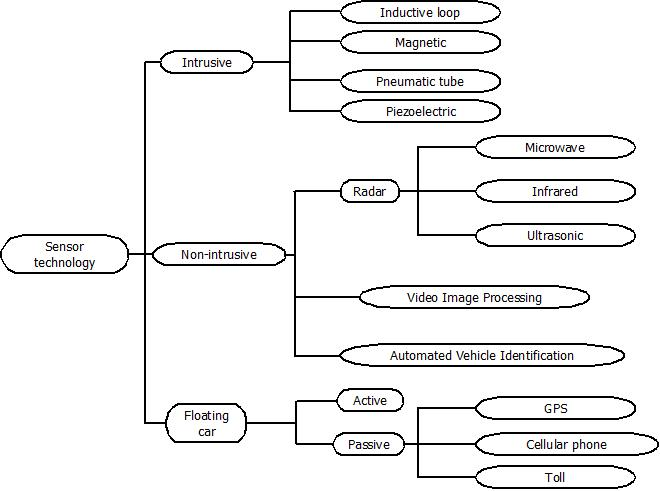
\includegraphics[scale=0.55]{intrusivos.jpeg}  %tipossensores.jpg}
\end{center} 
\caption{Information systems classification, according to the intrusiveness of the technology.} 
\label{tipossensores} 
\end{figure}

Main technologies currently used in traffic monitoring include pneumatic tubes, loop detectors, floating vehicles or automatic recognition systems, among others.


\emph{Manual counts} is the most traditional method. In this case trained observers gather traffic data that cannot be efficiently obtained through automated counts e.g. vehicle occupancy rate, pedestrians and vehicle classifications. The most common equipments used are tally sheet, mechanical count boards and electronic count board systems.

\emph{Passive and active infra-red} sensors are based on detecting the presence, speed and type of vehicles using the infrared energy radiating from the detection area. The main drawbacks are the performance during bad weather, and limited lane coverage.

\emph{Microwave radar} can detect moving vehicles and speed (Doppler radar). It records count data, speed and simple vehicle classification and is not affected by weather conditions.
\emph{Ultrasonic sensors} devices emit sound waves to detect vehicles by measuring the time for the signal to return to the device. They can be affected by temperature or bad weather. 

\emph{Pneumatic road tubes} are placed across the road lanes to detect vehicles from pressure changes that are produced when a vehicle tyre passes over the tube. The pulse of air that is created is recorded and processes by a counter located on the side of the road. The main drawback of this technology is that it has limited lane coverage and its efficiency is subject to weather, temperature and traffic conditions. This system may also not be efficient in measuring low speed flows.
\emph{Piezoelectric sensors} are very similar to pneumatic road tubes, although the principle is to convert mechanical energy into electrical energy. Indeed, mechanical deformation of the piezoelectric material modifies the surface charge density of the material so that a potential difference appears between the electrodes. The amplitude and frequency of the signal is directly proportional to the degree of deformation. This system can be used to measure weight and speed.

\emph{Magnetic loops} (inductive, magnetic, or video processing based) may be used temporarily or permanently, the latter being the more usual. 
It is the most conventional technology used to collect traffic data. The loops are embedded in roadways in a square formation that generates a magnetic field. The information is then transmitted to a counting device placed on the side of the road. This has a generally short life expectancy because it can be damaged by heavy vehicles, but is not affected by bad weather conditions. This technology has been widely deployed over the last decades. However, the implementation and maintenance costs can be expensive.

The use of so-called \emph{floating vehicles} consists on a vehicle provided with sensors to collect information while driving on a predefined route.
This active device data collection is one of the most popular among operators of roads, used especially for the collection of travel time and for loop detector calibration.
Depending on the level of automation in the data collection, the cost can vary.

In some areas, such as electronic toll or transit systems, \emph{automatic vehicle identification systems} (AVI) are also widely used. 
These sensors are non-exhaustive data sources to identify tags located in vehicles, such as in payment-systems without stopping. 
The system detects the pass, and the data is sent to the server to be processed to perform an event (pay toll, opening in the fence, etc).

The main disadvantage of these systems is that they are unable to identify vehicles detected, in order to obtain origin/destination matrixes.
Just the number of vehicles and their type can be calculated, but does not allow to obtain moves flow, nor to determine whether a certain vehicle passes repeatedly.
In addition, its high cost makes it unprofitable covering secundary roads with them, so they are often located on major roads.

Finally, the \emph{automatic recognition} technology has experienced an increase in recent years due to its ability to detect individual vehicles without relying on in-vehicle systems. 
Video image detection is a good example: video cameras record vehicle numbers, type and speed by means of different video techniques e.g. trip line and tracking. 
Furthermore, they are used for automatic detection of incidents on the road. 
That is the main advantage over previous information systems.
However, system reliability might not be the best, as the system can be sensitive to meteorological conditions.
Moreover, these systems are very costly compared to the previous.
Finally, from a privacy point of view, the Spanish Data Protection Agency (Agencia de Protección de Datos) considers the car license plate as a personal data, so that it would require the user consent.




\subsection{Commercial products}
There are different companies working in the traffic information area using approaches similar to the presented in this work.

\begin{itemize}

\item \textbf{Bit Carrier} \cite{patenteBC} \cite{BitCarrier}: It offers a traffic management system based in BT to count people and commercial routes (pathsolver). Its technology was implanted in highways managed by Abertis for traffic control and monitoring. Actually it has a 150 devices network in Catalonia, so it allows count the traffic times of 200.000 persons each day.
 
\item \textbf{Trafficnow} \cite{Trafficnow}: Another BT system product. A pilot experience has been implanted in Vigo.

 \item \textbf{Traffax Inc} \cite{TraffaxInc}: It is a company that also has used BT for calculating origin-destination and transport time matrixes.

 \item \textbf{Savari Networks} \cite{SavariNetworks}: It offers the commercial product StreetWAVE for traffic monitoring to know in real time the traffic status.


 \item \textbf{TrafficCast} \cite{TrafficCast}: They have developed prediction models in different cities based on different technologies, such as cameras, BT and RFID included in the vehicles.

\end{itemize}

The proposal presented in this work have some common features with the previous approaches, offering similar functionalities with reduced cost.


%%%%%%%%%%%%%%%%%%%%%%%%%%%%%%%%%%%%%%%%%%%%%%%%%%%%%%%%%%%%%%
\section{Objectives and expected results}
\label{obj}

The main objective is building a low-cost system, with a fast implantation and highly reliable. 
It will provide real-time information about the traffic status, not only to the official organisms and agencies in charge of the traffic controlling, but also to any person who requests it (available as web services).

Several features have been developed:

\begin{itemize}
  \item \textit{Data collection component}: it includes several sensors to continuously scanning and identify BT devices. It uses a 3G connection to send data the storage server.
  
  \item It is enclosed in hermetic boxes, with a power line (220volt).

  \item \textit{Data processing component}: it stores the obtained data, and offers some tools to serve them (through web services).

  \item \textit{Information service}: it provides the users the requested information related to the traffic status.
\end{itemize}

Thus, six devices were installed for data collection. They send obtained data to servers for further data processing. 
Node locations is detailed in Table \ref{localizaciones}, and shown in the map on Figure \ref{mapa}.
Locations were set according to the suggestions of DGT staff, looking for an adequate place, with a continuous flow of vehicles, and also taking into account the assembly difficulty of the monitoring devices.

 \begin{table}
 \begin{center}
 \begin{tabular}{|c|l|}
 \hline
Node Id.  &  Location      \\
 \hline
    1     &  C/ Julio Verne, 2    \\
 \hline
    2     &  C/ Calle del Periodista Daniel Saucedo, s/n    \\
 \hline
    3     &  Plaza del Duque, s/n    \\
 \hline
    4     &  Autovía de Sierra Nevada, km 119,550    \\
 \hline
    5     &  Autovía de Sierra Nevada, km 123,250    \\
 \hline
    6     &  C/ Calle Goleta, 1    \\
 \hline
 \end{tabular}
 \end{center}
 \caption{Node locations.
 \label{localizaciones}}
 \end{table}

Additionally, a website has been created, including an information panel allowing different consults about the traffic state on the monitored zone.

\begin{figure}[htpb] 
\begin{center} 
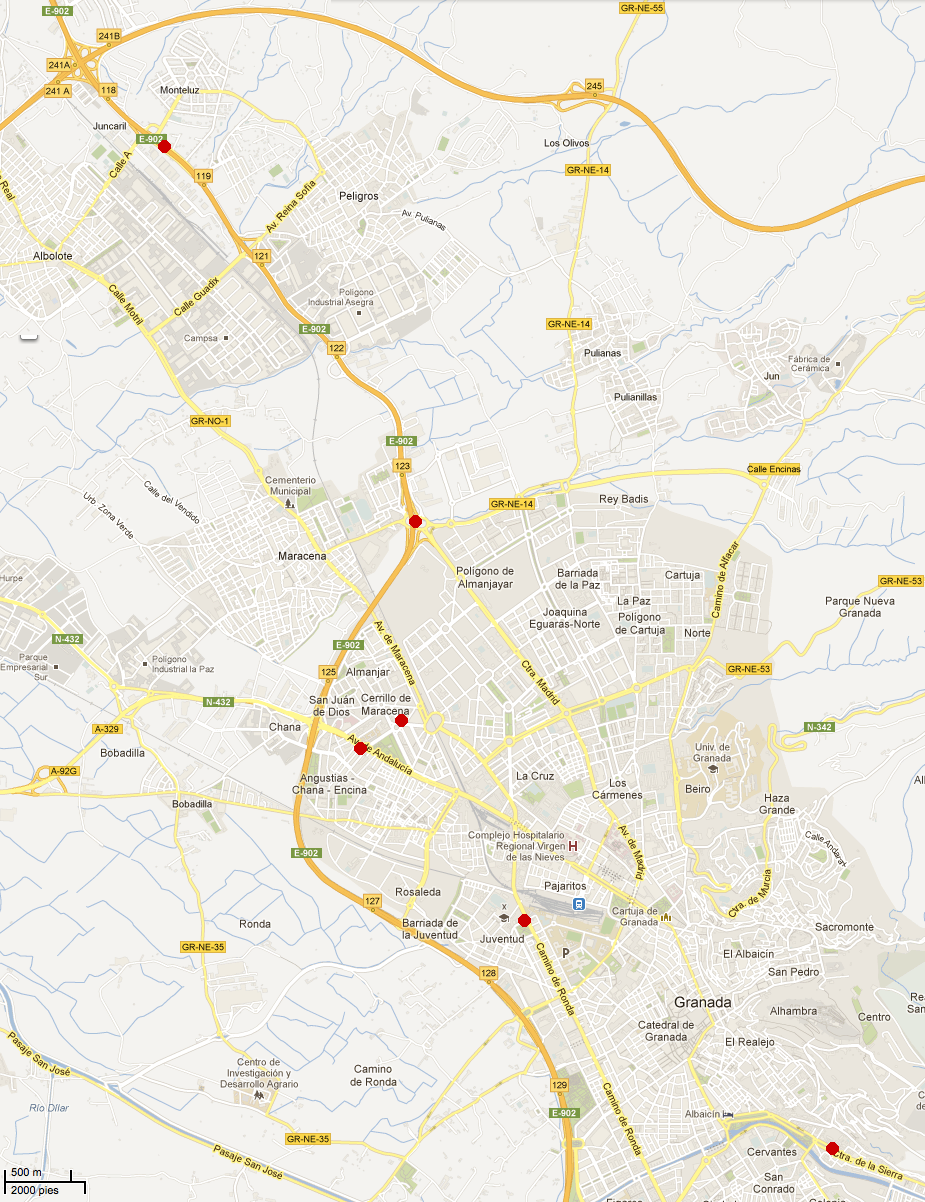
\includegraphics[scale=0.35]{mapa.png}
\end{center} 
\caption{Geographical node locations in the metropolitan area of Granada. Source http://bit.ly/SQdQkH} 
\label{mapa} 
\end{figure}

We expect collecting a large amount of data corresponding to passing BT devices, to populate a big database and to compute different statistics and indicators on the use of vehicles on the monitored area, driving habits and even the effect of important factors or events (key dates, nonworking days, etc).

Specifically, following statistics will be reported:

\begin{itemize}
 \item total amount of vehicles detected by every node
 \item total amount of vehicles detected in working days
 \item total amount of vehicles detected in non-working days
 \item number of times each vehicle is detected
 \item type of path that the vehicles follow
 \item traffic density by time range and road type
 \item average speed in the road where two devices where set
\end{itemize}

Finally, an important event has been analysed, since on November 14th there was a general strike day in Spain, so some conclusions about traffic changes that day would be studied.


%%%%%%%%%%%%%%%%%%%%%%%%%%%%%%%%%%%%%%%%%%%%%%%%%%%%%%%%%%%%%%
\section{Data-collecting hardware device}
\label{hw}

The first step of the study is to choose between several hardware devices to scan for BT devices in range. First test were conducted on a PC with Linux and a BT module. This solution was quickly discarded because of its high size and power consumption were a problem.

Another possible solution studied were using cell phones with Android due to its high autonomy based on low power consumption, high connectivity, highly available development tools and processor been powerful enough.

A prototype application\footnote{Application available for download at the address http://bit.ly/VY5kR6} was developed for Android. The application was limited to three task: BT device discovery, BT identification data saving to a text file in the cell phone memory and data sending to a server thorough its 3G connection. The server finally stores the information about the BT devices on a database. Several screenshots of the application running can be seen on Figure \ref{apk}.

\begin{figure}[htpb] 
\begin{center} 
\begin{tabular}{cc}
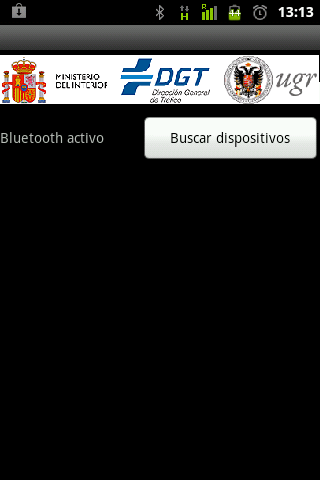
\includegraphics[scale=0.3]{CAP1.png}  &
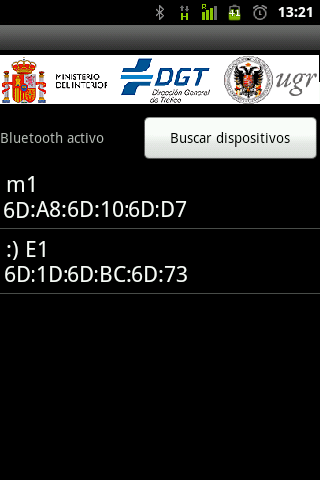
\includegraphics[scale=0.3]{CAP2.png}  \\
a & b 
\end{tabular}
\end{center} 
\caption{Screenshots of the Android application that was developed for BT device discovery. a) Application ready for discovery. b) Application while discovering BT devices.} 
\label{apk} 
\end{figure}

Despite the advantages of the cell phone, the integrated BT devices are low power and small antennas are used because of the power limits. After comparing the detection capability of the cell phone with the PC with and external BT device, the cell phone was discarded.

Thus a third solution was sought with a low power consumption and a high detection range in mind. Finally the Intelify \cite{intelify} (see Figure
\ref{intelify}) was chosen.

\begin{figure}[htpb] 
\begin{center} 
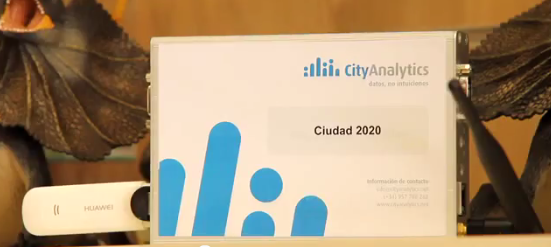
\includegraphics[scale=0.5]{intelifychisme1.png}
\end{center} 
\caption{Intelify device with a connected USB 3G dongle.} 
\label{intelify} 
\end{figure}

Intelify is a hardware detection device based on technology developed by Ciudad 2020 \cite{cityanalytics,Blobject}. It is an autonomous unit who scan the enviroment and sends the information to a central server for further processing and interpretation. Table \ref{caracteristicas} shows main features of the device.

\begin{table}[htpb]
\begin{center}
\begin{tabular}{|c|c|}
\hline
Dimensions & 113x163x30mm \\
\hline
     & Power             \\
LEDs & 3G activity       \\
     & Ethernet activity \\
\hline
           & Ethernet  \\
Networking & Wireless  \\
           & Bluetooth \\  
           & 3G        \\
\hline
USB ports & City Analytics Antenna \\
		  & 3G dongle              \\
\hline
Other ports & RS-232 \\
			& VGA    \\
\hline
 	  & 18v - 1200mA          \\
Power & external jack - 5.5mm \\
      & internal jack - 2.1mm \\
\hline
Network     & Ethernet RJ45 \\
connections & 3G USB Modem  \\
\hline
Antennas & City Analytics USB antenna \\
		 & wireless antenna \\
\hline
Microphone & noise sensor \\
\hline
Temperature & main board temperature sensor with extrapolation \\
\hline
Box & 1.5mm aluminum box \\
    & external use possible  \\
\hline
Operating System & Debian 6.0 Squeeze  \\
\hline
\end{tabular}
\end{center}
\caption{Main features of the Intelify device.}
\label{caracteristicas}
\end{table}

Intelify is a small autonomous computer that can be installed in any area to be monitored. 
It has several sensors that let you discover what is happening in its sorroundings like the flow of people and vehicles.

% http://www.numerodepersonas.com  \cite{numerodepersonas}
% http://www.cityanalytics.net/?act=faq  \cite{cityanalytics}

Technology was developed by Ciudad 2020 and the services offered are based on a net of Intelify devices with the capacity to discover information about the physical enviroment and help with decision making to any kind of organization based on people flow and behavior.

Valuable information about tourism, trade and mobility can be gathered through the deployment of autonomous devices around a city. A specific example is the service offered in \cite{numerodepersonas}. It offers information about foot traffic through Cordoba city center.

The cost of this solution is 1000 euros per device, including maintenance of remote computer, communications using a 3G telephony service and storage and data management.

Data accuracy is very representative, compared against other technologies.
In \cite{estudioprecision} it was obtained an a priori error estimation of $8.5\%$ of detections.
%This study \cite{estudioprecision} shows that the average error found in the detection of people is 8.5\%.




%%%%%%%%%%%%%%%%%%%%%%%%%%%%%%%%%%%%%%%%%%%%%%%%%%%%%%%%%%%%%%
\section{Data analysis}
\label{analisis}


 % En esta sección se llevan a cabo diversos análisis de los datos recopilados durante el periodo de monitorización (del 8 de noviembre al 9 de diciembre) para obtener estadísticas y así estudiar el uso de vehículos.
In this section the analysis of collected data during the monitoring period (November 8 to December 9) to obtain statistics and so study the use of vehicles is carried out.

 % Concretamente, en las siguientes subsecciones, reportaremos información acerca del número total de vehículos detectados por cada nodo, en días laborables o festivos, sobre la densidad del tráfico por rango horario, acerca de los desplazamientos individuales, y de la velocidad media en un tramo delimitado por dos nodos consecutivos.
Specifically, the following subsections report information about the total number of vehicles detected by each node, on weekdays or holidays, information on traffic density by time range on individual movements, and the average speed on a section delimited by two consecutive nodes.

 % Por último, puesto que el día 14 de noviembre de 2012 se celebró la huelga general, estudiaremos cómo afectó la huelga al tráfico en el área metropolitana de Granada, comparando los totales de detección de dispositivos entre el día de la huelga (14 de noviembre), y el miércoles siguiente (21 de noviembre).
Finally, since November 14 2012 a general strike was held, we will study how the strike affected traffic in the metropolitan area of Granada (Spain), by comparing total number of devices detected that day (November 14), and the following day (November 15).


\subsection{Total number of vehicles detected (weekdays and holidays)}
 % VehiculosTotales.txt tiene los vehículos totales detectados en cada nodo.

% La primera parte del análisis ha consistido en calcular el número de dispositivos detectados por cada uno de los nodos instalados.
The first analysis consisted in calculating the number of devices detected by each node.

 \begin{table}
 \begin{center}
 \begin{tabular}{|c|c|}
 \hline
Node Id.  &  N. of devices detected  \\
 \hline
    1     &    31408  \\
 \hline
    2     &    45032  \\
 \hline
    3     &    33165  \\
 \hline
    4     &    358494  \\
 \hline
    5     &    297874  \\
 \hline
    6     &    7872  \\
 \hline
 \end{tabular}
 \end{center}
 \caption{Number of BT devices detected by each node.
 \label{VehiculosTotales}}
 \end{table}

 % En total se han detectado 773845 dispositivos BT al paso por los seis nodos. 
 % Como se observa en la Tabla \ref{VehiculosTotales}, los dos nodos situados en la autovía de Sierra Nevada (A44, Circunvalación de Granada, nodos 4 y 5) son los que más datos han recogido, mientras que el situado en una calle secundaria (nodo 6) ha sido el que menos dispositivos ha recogido.

In total, 773,845 BT devices have been detected by the six nodes.
As shown in Table \ref{VehiculosTotales}, nodes located in the Sierra Nevada Highway (A44, nodes 4 and 5) have collected a higher number of data, while the node located in a side street (node 6) has detected the smallest number of devices.


\subsection{Total vehicles detected on non-working days}
 % VehiculosFestivos.txt tiene los vehículos detectados en día festivo en cada nodo.

 % A continuación, y para comparar la intensidad circulatoria entre días laborables y no laborables, se ha calculado el número de pasos en días festivos y no laborables.
To compare the traffic intensity between working and non-working days, the number of pass on holidays and non-working days have been obtained.

 \begin{table}
 \begin{center}
 \begin{tabular}{|c|c|}
 \hline
Node Id.  &  N. of devices detected  \\
 \hline
    1     &    2149  \\
 \hline
    2     &    2804  \\
 \hline
    3     &    2832  \\
 \hline
    4     &    32182  \\
 \hline
    5     &    24166  \\
 \hline
    6     &    1269  \\
 \hline
 \end{tabular}
 \end{center}
 \caption{Total number of BT devices detected by each node (only on non-working days).
 \label{VehiculosFestivos}}
 \end{table}

 % La Tabla \ref{VehiculosFestivos} muestra un descenso en el número de dispositivos detectados por todos los nodos en días no laborables, frente al número de detecciones en días laborables. 
 % Aún así, los nodos situados en la autovía de Sierra Nevada siguen recogiendo muchos más datos que el resto, debido al tráfico denso que soporta esta vía en días no laborables.

Table \ref{VehiculosFestivos} shows how the number of detected devices lowers by all nodes on non-working days, compared to the number of detections on weekdays.
Nodes located in the Sierra Nevada Highway still collected much more data than the remainder, due to the traffic this road supports on holidays.


\subsection{Traffic density on the road by time range}
 % VehiculosDiferentesPorHoras.txt contiene para cada uno de los nodos, los dispositivos diferentes detectados en cada rango horario (final de la línea)

 % La densidad circulatoria por horas podemos calcularla a partir del total de dispositivos diferentes detectados en cada rango horario.
Traffic density can be calculated taking into account the total number of detected devices by time range.

 \begin{figure}[htb]
 \begin{center}
 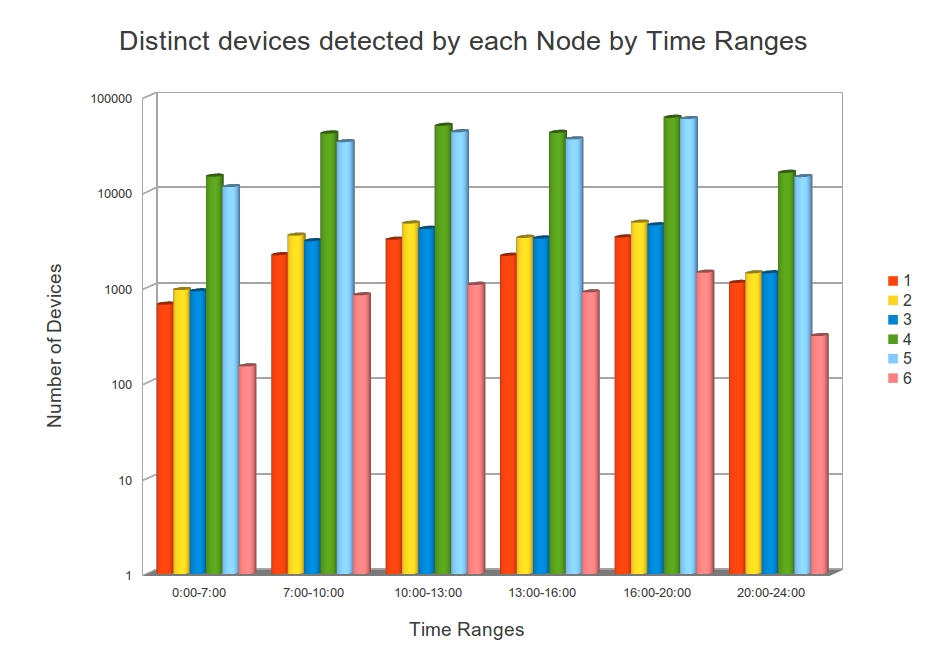
\includegraphics[scale=0.4]{VehiculosDiferentesPorHoras.jpg}
 \caption{For each node, the total number of different detected devices by time range is shown. Figure is shown in logarithmic scale.
 % Para cada uno de los nodos se muestra el total de dispositivos diferentes detectados en cada rango horario. Para cada rango de horas se muestra el total detectado en cada uno de los seis nodos
 \label{VehiculosDiferentesPorHoras}}
 \end{center}
 \end{figure}
 % Gráfica (histograma) de la densidad de la vía por horas: desde las 00-7h, de 7-10h, de 10-13h, de 13-16h, de 16-20h, y de 20-24h.
 
 % La Figura \ref{VehiculosDiferentesPorHoras} muestra mayor densidad, en todos los nodos, a las horas punta de entrada o salida del trabajo y colegios.
Figure \ref{VehiculosDiferentesPorHoras} shows higher density on all nodes, at peak times or out of work and school.


\subsection{Total detections by time range}
 % VehiculosPorHoras.txt indica para cada nodo, el número de dispositivos detectados en el rango horario, sin diferenciar si el dispositivo es siempre el mismo o no. 

 % Adicionalmente podemos calcular para cada nodo, el número de dispositivos detectados en cada rango de horas, sin diferenciar si el dispositivo es siempre el mismo o no. Así pues, se incluirán pasos repetidos del mismo vehículo.
Additionally we can calculate for each node, the number of detected devices by time range, without differentiating whether the device is the same or not (repeated passes). Thus, repeated passes of the same vehicle are counted.

 \begin{figure}[htb]
 \begin{center}
 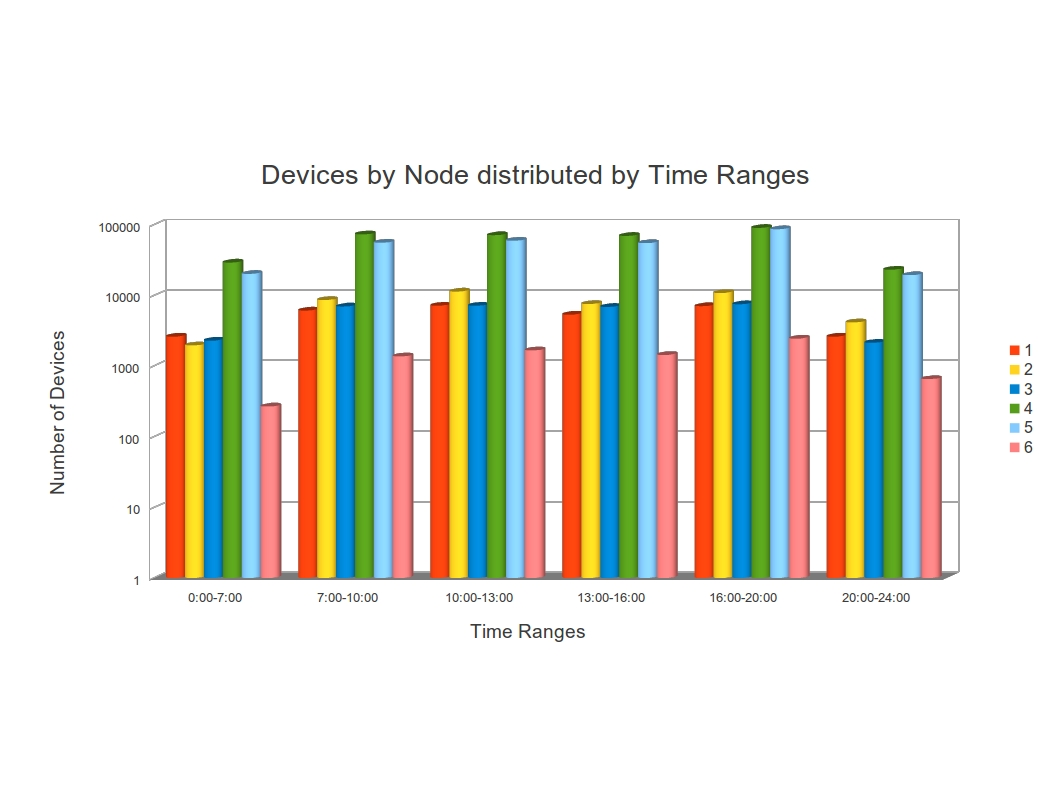
\includegraphics[scale=0.4]{VehiculosPorHoras.jpg}
 \caption{For each of the six nodes, the total number of detected devices by time range is shown. Figure is shown in logarithmic scale.
 % Para cada uno de los nodos se muestra el total de dispositivos detectados en cada rango horario. Para cada rango de horas se muestra el total detectado en cada uno de los seis nodos
 \label{VehiculosPorHoras}}
 \end{center}
 \end{figure}
 
 % Al igual que en el caso anterior, observamos una mayor densidad circulatoria en todos los nodos, a las horas punta de entrada o salida del trabajo y colegios (ver la Figura \ref{VehiculosPorHoras}).
As in the previous case, a greater traffic density can be observed on all nodes, at peak times or out of work and school. (see Figure \ref{VehiculosPorHoras}).


\subsection{Number of individual vehicles detections}
 % Intervalos.txt contine el número de vehículos detectados entre 0 y 5 veces, entre 5 y 10 veces y así sucesivamente hasta más de 25 veces detallado en cada nodo.

 % A continuación podemos sacar partido de la capacidad del sistema propuesto para individualizar los dispositivos BT, pudiendo detectar si esos mismos vehículos repiten paso por diferentes nodos.
We can take advantage of the proposed system's ability to identify BT devices. Thus, it can be detected whether vehicles pass by different nodes.

 \begin{figure}[htb]
 \begin{center}
 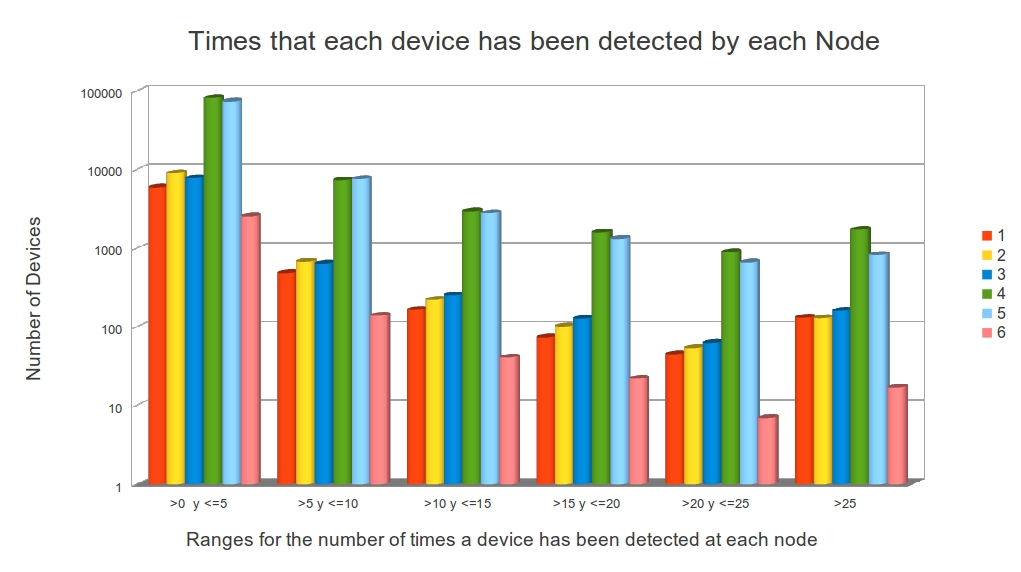
\includegraphics[scale=0.4]{Intervalos.jpg}
 \caption{For each of the six nodes, the total number of detected devices N times (repeated occurrences of the same device) are shown. Figure is shown in logarithmic scale.
 % Para cada uno de los nodos se muestra el total de dispositivos detectados cierto número de veces (repetidas apariciones del mismo dispositivo)
 \label{Intervalos}}
 \end{center}
 \end{figure} 
 % Histograma que muestre cuántos coches se detectan entre una y 5 veces, entre 6 y 10, entre 10 y 20, y más de 20 veces.

 % En la Figura \ref{Intervalos} podemos ver que hay una gran cantidad de vehículos que repiten su paso por ciertos nodos (principalmente los situados en la A44) hasta 10 veces. 
 % Incluso se puede ver que en los nodos 4 y 5 hay alrededor de 1000 vehículos que repiten su paso más de 25 veces. En el resto de nodos, más de 25 repeticiones del mismo dispositivo se han detectado alrededor de 120 veces solamente.

Figure \ref{Intervalos} shows a large number of vehicles that pass repeated times (up to 10 times) by some of the nodes (mainly those located in the A44).
Even it can be seen that nodes 4 and 5 detect about 1,000 vehicles passing more than 25 times repeated. 
On the other nodes, over 25 repetitions of the same device have been detected only around 120 times.


\subsection{Complexity of displacement}
 % NodosPorDondePasan.txt contiene el número de vehículos que han pasado por 2 nodos, por 3 nodos y así hasta por los 6 nodos y el número medio de veces que han pasado 2, 3, 4, 5 o 6 veces por cada nodo.

 % En el estudio de la complejidad de los desplazamientos se han calculado el número de vehículos que han pasado por 2 nodos, por 3 nodos y hasta 6 nodos. En la Tabla \ref{tNodosPorDondePasan} se muestra además el número medio de veces que han pasado un vehículo por 2, 3, 4, 5 o 6 nodos.
To study the complexity of displacements, the number of vehicles that have passed through two nodes, 3 nodes and up to 6 nodes  were calculated. 
Table 4 also shows the average number of times that vehicles have passed through 2, 3, 4, 5 or 6 nodes.

 \begin{table}
 \begin{center}
 \begin{tabular}{|c|c|c|c|}
 \hline
 No. of nodes & 	No. of devices & 	Total number of passes & 	Mean $\pm$ std. dev.  \\
 \hline
1 & 	72989 & 	 165033 & 	$2.26 \pm 31.16$  \\
 \hline
2 & 	53947 & 	 425667 & 	$7.89 \pm 11.48$  \\
 \hline
3 & 	8125 & 	 131570 & 	$16.19 \pm 24.71$  \\
 \hline
4 & 	1359 & 	 39241 & 	$28.88 \pm 140.82$  \\
 \hline
5 & 	254 & 	 8603 & 	$33.87 \pm 59.51$  \\
 \hline
6 & 	61 & 	 3731 & 	$61.16 \pm 94.78$  \\
 \hline
 \end{tabular}
 \end{center}
 \caption{Total number of vehicles that have passed through two nodes, 3 nodes and up to 6 nodes, and average number of times that vehicles have passed through 2, 3, 4, 5 or 6 nodes. In some cases the deviations are high because some devices have a very high number of occurrences for some nodes.
 % Número de vehículos que han pasado por 2 nodos, por 3 nodos y hasta 6 nodos, y el número medio de veces que han pasado los vehículos por 2, 3, 4, 5 o 6 nodos. En algunos casos las desviaciones son altas debido a que algunos dispositivos tienen un número muy alto de apariciones por algunos de los nodos
 \label{tNodosPorDondePasan}}
 \end{table}

 % La información anterior se complementa visualmente con la Figura \ref{fNodosPorDondePasan}, en la que se muestra (en escala logarítmica) cuántos coches pasan sólo por un nodo, por dos nodos, por tres nodos, etc.
The above information is complemented with Figure \ref{fNodosPorDondePasan}, that shows how many cars pass by only one node, two nodes, three nodes, etc.

 \begin{figure}[htb]
 \begin{center}
 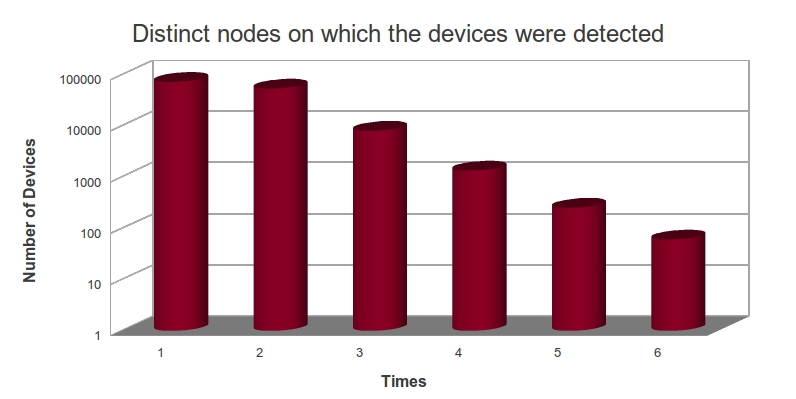
\includegraphics[scale=0.4]{NodosPorDondePasan.jpg}
 \caption{Figure shows how many cars pass by only one node, two nodes, three nodes, etc. Figure is shown in logarithmic scale.
 % La figura muestra cuántos coches pasan sólo por un nodo, por dos nodos, por tres nodos, etc. Para mejorar la visualización se ha utilizado escala logarítmica
 \label{fNodosPorDondePasan}}
 \end{center}
 \end{figure}
 % Histograma que muestre cuántos coches pasan sólo por un nodo, por dos nodos, por tres nodos, etc.

 % Como se esperaba, gran parte de los dispositivos BT pasan pocas veces por casi todos los nodos, mientras que la mayoría pasa sólo por uno o dos de ellos (sus desplazamientos se centran en una parte de la zona pequeña monitorizada).
As expected, most of the BT devices rarely passed by all nodes, while most of devices pass only by one or two of nodes (their displacements are focused on a small part of the monitored area).


\subsection{Effect of Nov-14 strike on zone traffic}
 % Tabla en la que mostremos cómo afectó el día 14-N con la huelga.

 % Justo en mitad del periodo de monitorización, en España se celebró un día de huelga general (14 de noviembre de 2012), lo que ha quedado reflejado en la cantidad de coches detectados en los nodos.

 % Se ha analizado el efecto de la huelga general en el tráfico de la zona monitorizada, mostrando en la Tabla \ref{huelga} el número de pasos detectados el día 14 de noviembre y justo el día siguiente.

Right in the middle of the monitoring period in Spain was held a day of general strike (November 14, 2012), which has been reflected in the number of detected devices (cars) on the nodes.

The effect of the general strike in the traffic of the monitored area has been analyzed and shown in Table \ref{huelga} as the number of detected devices on November 14 and the very next day.

 \begin{table}
 \begin{center}
 \begin{tabular}{|c|c|c|}
 \hline
 Node  &  Total number of passes (nov-14) & Total number of passes (nov-15) \\
 \hline
 2	& 1841  & 2722  \\
 \hline
 3	& 891   & 1169 \\
 \hline
 4	& 10807	& 16942 \\
 \hline
 5	& 831  	& 4017\\
 \hline
 6	& 946   & 1419 \\
 \hline
 \end{tabular}
 \end{center}
 \caption{Comparison of the number of passes for each node between the general strike day (November 14) and the very next day. Node 1 results are not reported because the hardware device suffered a power supply problem for a couple of days at that time.
 % Comparación del número de pasos por cada nodo entre el día de la huelga general (14 de noviembre) y el día siguiente. No aparece recogido el nodo 1 debido a que el dispositivo hardware sufrió un problema de alimentación durante un par de días en esas fechas
 \label{huelga}}
 \end{table}

 % En la Tabla \ref{huelga} se aprecia un número de vehículos detectados menor el día de la huelga respecto al día siguiente (laborable en el que la actividad debió ser normal en la zona).
Table 8 shows a lowest number of detected vehicles the day of the strike that on the following day (working day in which the activity should be normal in the area).


\subsection{Analysis of vehicles speed between two consecutive nodes}
 % tabla de la velocidad media de los vehículos en el tramo (en laborables y en fin de semana).
 % El "Granada 5" está en el km 123,250 ; el "Granada 4" está en el km 119,550 ; hay 3700 metros entre ambos. 

 % Por último, a partir de los dos nodos consecutivos localizados en la autovía A44, podemos calcular velocidades medias en el tramo delimitado por los nodos 4 (situado en el km 119,550) y 5 (situado en el km 123,250) de un total de 3700 metros. 
 % En realidad podemos calcular la velocidad media en el tramo a nivel global, no la velocidad a la que ha ido cada vehículo en cada instante dentro del tramo.

Finally, taking two consecutive nodes, located on the A44 highway, average speeds in the section bounded by nodes 4 (located at km 119.550) and 5 (located at km 123.250) can be calculated.
This highway section where the study takes place is of 3700 meters long.
Actually, we can calculate the average speed in the global section, not the speed at which each vehicle has at each instant within the section.

 \begin{table}
 \begin{center}
 \begin{tabular}{|c|c|}
 \hline
Speed range (km/h) &  No. of passes  \\
 \hline
v$\leq$60.0	& 1495  \\
 \hline
60.0$\leq$v$\leq$70.0 & 2585  \\
 \hline
70.0$\leq$v$\leq$80.0 & 7421  \\
 \hline
80.0$\leq$v$\leq$90.0 & 16339  \\
 \hline
90.0$\leq$v$\leq$100.0 & 20144  \\
 \hline
100.0$\leq$v$\leq$120.0 & 14384  \\
 \hline
120.0$\leq$v$\leq$140.0 & 5434  \\
 \hline
v$\geq$140.0 & 1326  \\
 \hline
 \end{tabular}
 \end{center}
 \caption{Average speeds (globally) in the section bounded by nodes 4 and 5.
  % Velocidades medias (a nivel global) en el tramo delimitado por los nodos 4 y 5
 \label{velocidad}}
 \end{table}


 % En dicho tramo, la velocidad está limitada a 100 km/h. Sin embargo, y aunque la gran mayoría respetan el límite, vemos que una gran cantidad de coches superan dicha limitación.
In that section, the speed is limited to 100 km/h. However, although most of the vehicles respect this limit, a lot of cars exceed this limitation.


%%%%%%%%%%%%%%%%%%%%%%%%%%%%%%%%%%%%%%%%%%%%%%%%%%%%%%%%%%%%%%
\section{Conclusions and future work}
\label{conclus}

 %% Estudio de los indicadores de exposición en el área metropolitana de Granada mediante un nuevo sistema de información de bajo coste
 %% Obtención de indicadores de exposición mediante un nuevo sistema de información de bajo coste

%Los sistemas de información utilizados actualmente para la recopilación de datos sobre el estado de 
% las carreteras carecen de la capacidad para individualizar los vehículos que detectan, 
% o bien presentan un elevado coste.
The information systems currently used for collecting data about the road conditions are not able to uniquely identify detected vehicles, and if they do, these information systems have a high cost.

%En este trabajo se ha presentado un nuevo sistema de información de bajo coste para monitorizar el tráfico en diferentes tipos de vías en tiempo real.
This paper presents a new low-cost information system to monitor traffic on different road types and in real time.

%El objetivo principal ha sido en todo momento la obtención de indicadores de exposición mediante un nuevo sistema basado en la detección de dispositivos BT que pasan por diferentes nodos de información.
The main goal was getting exposure indicators using a new system based on the BT devices detection using several collecting nodes.


%De esta forma, hemos podido monitorizar la densidad de tráfico y los desplazamientos realizados por los usuarios, individualizando los vehículos conforme se mueven entre nodos dentro de la zona.
Thus, we are able to monitor the traffic density and car journeys, identifying the vehicles when they move from one nodo to another inside the monitored zone.

%Así pues, se han estudiado diferentes soluciones para desarrollar un dispositivo hardware de detección, habiendo descartado algunas por costosas, por su alto consumo o por su corto alcance en el escaneo.
Moreover, different hardware solutions have been studied to carry out device detection, and we have rejected some of them for its high prices, for its energy inefficiency or for their short-range for detection.


%Además, se han tenido en cuenta diferentes tipos de vía, con muy distintos tipo de tráfico. 
%También se han obtenido estadísticas en función de los días de la semana y de los horarios de circulación.
Also we have taken into account different road types, with different traffic type.
Statistical data have also been obtained grouped by days of the week and hours of day.

%Se han realizado diversos análisis de los datos recopilados durante el periodo de monitorización (del 8 de noviembre al 9 de diciembre de 2012) para obtener diferentes estadísticas.
Several statistics of the collected data have been calculated during the monitoring period (November 8th to December 9th, 2012).


%Concretamente, se ha estudiado el número total de vehículos detectados por cada nodo, en días laborables o festivos. También se ha estudiado la densidad del tráfico por rango horario, y los desplazamientos individuales.
Specifically, the total number of BT detected devices by each node has been analysed, on holidays or working days. 
We also have analysed the traffic density by time range, and the journeys of the drivers in the monitored zone.

%Por último, se ha analizado la velocidad media en un tramo delimitado por dos nodos consecutivos.
Then, average speed of some journeys has been calculated for a set of drivers that were detected by two consecutive nodes in the highway.

%Finalmente, ha quedado demostrada la potencia y funcionalidad del sistema, que se complementa con el desarrollo de un conjunto de servicios web para facilitar el acceso a la información en tiempo real, pudiendo realizar diferentes tipos de consultas.
Finally, the power and features of the system have been demostrated. This has been complemented by developing a set of web services for easy access to the data in real time, including different statistics.

%Como trabajos futuros se abren diversas líneas de investigación, centradas principalmente en el procesamiento de los datos recogidos mediante algoritmos complejos de minería de datos \cite{Trevor2009}, computación evolutiva \cite{Eiben2003,Michalewicz2004,Yang2010} y redes neuronales \cite{Castillo2001,Rivas2003,Castillo2007}, aprendizaje automático \cite{Arenas2005} y de métodos estadísticos \cite{Jiawei2006,Hill2007,Nisbet2009}, que se irán desarrollando e integrando como servicios web \cite{Papazoglou2007,pgs2007} en el sistema.
Several future research lines have been opened, they are mainly focused on processing the collected data using data mining algorithms \cite{Trevor2009}, evolutionary computation methods \cite{Eiben2003,Michalewicz2004,Yang2010}, artificial neural networks \cite{Castillo2001,Rivas2003,Castillo2007}, machine learning models \cite{Arenas2005} and statistical methods \cite{Jiawei2006,Hill2007,Nisbet2009}, which will be included and integrated as web services \cite{Papazoglou2007,pgs2007} in the system.

%La idea es desarrollar en el futuro un sistema de predicción y ayuda a la toma de decisiones, capaz de aplicar conocimiento en aplicaciones relacionadas con la movilidad. 
Our purpose is to develop in the future a prediction system that helps to make decisions, and able to apply knowledge in applications related to mobility.


%Se espera que el desarrollo e implantación de este tipo de sistemas ofrezca una serie de servicios de información con valor añadido que no se consiguen con las tecnologías actuales.
It is expected that the development and deployment of these systems will offer a set of information services with added value that are not achieved with current technologies.

%\newpage

\bigskip

%%%%%%%%%%%%%%%%%%%%%%%%%%%%% AGRADEC. %%%%%%%%%%%%%%%%%%%%%%%%%%%%%%%%%%%
\section*{Acknowledgements}

This work has been supported by the \emph{SISTEMA DE INFORMACIÓN DE BAJO COSTE PARA CONOCER EL ESTADO DE LAS CARRETERAS EN TIEMPO REAL}
(Expediente de contratación 0100DGT21285) 
project of the Spanish Dirección General de Tráfico.
 

% \begin{figure}[htb]
% \begin{center}
% \includegraphics[scale=0.4]{figura.png}
% \caption{Texto de la figura. 
% \label{ejfigura}}
% \end{center}
% \end{figure}


% \begin{table}
% \begin{center}
% \begin{tabular}{|c|c|c|c|}
% \hline
% col1  & col2 & col3 & col4  \\
% \hline
% col1  & col2 & col3 & col4  \\
% \hline
% col1  & col2 & col3 & col4  \\
% \hline
% \end{tabular}
% \end{center}
% \caption{Texto de la tabla
% \label{ejtabla}}
% \end{table}


%%%%%%%%%%%%%%%%%%%%%%%%%%%%%%%%%%%%%%%%%%%%%%%%%%%%%%%%%%%%%%%%%%%%%%%%%
%%%%%%%%%%%%%%%%%%%%%%%%%%%%%%%%%%%%%%%%%%%%%%%%%%%%%%%%%%%%%%%%%%%%%%%%%
\bibliographystyle{unsrt}
\bibliography{referencias}
\end{document}
